We used \glspl{esn} to forecast electricity demand, or electric load, both
4 hour intervals and 48 hour intervals. Figure \ref{fig:48demand} shows the
48-hour ahead forecast that had the lowest RMSE. In this case, the forecast
that used relative humidity as an additional input had the lowest error, as
shown in Table \ref{tab:demand48}. Table \ref{tab:demand48} also shows that the
forecast was weakened by training with air temperature (both wet bulb and dry
bulb), air pressure, and wind speed. Adding solar elevation angle performed
about the same as the base case.

The 4-hour interval forecast with the lowest
RMSE is shown in Figure \ref{fig:demand04}. Solar elevation angle improved the
forecast more than any other meteorological input. Table \ref{tab:demand04}
shows that humidity, air pressure, dry bulb temperature, and wind speed made the
forecast worse.

The performance of this implementation is consistent with previous applications
of \glspl{esn} to the task of predicting electric load
\cite{deihimi_application_2012}. Further, these results indicate that
\glspl{esn} perform better than other machine learning techniques -- long
short term memory (LSTM)\cite{marino_building_2016}, Sequence to Sequence (S2S)
\cite{marino_building_2016}, and support vector regression \cite{chen_day-ahead_2017} -- for predicting energy demand.

\begin{figure*}[h]
  \centering
  % 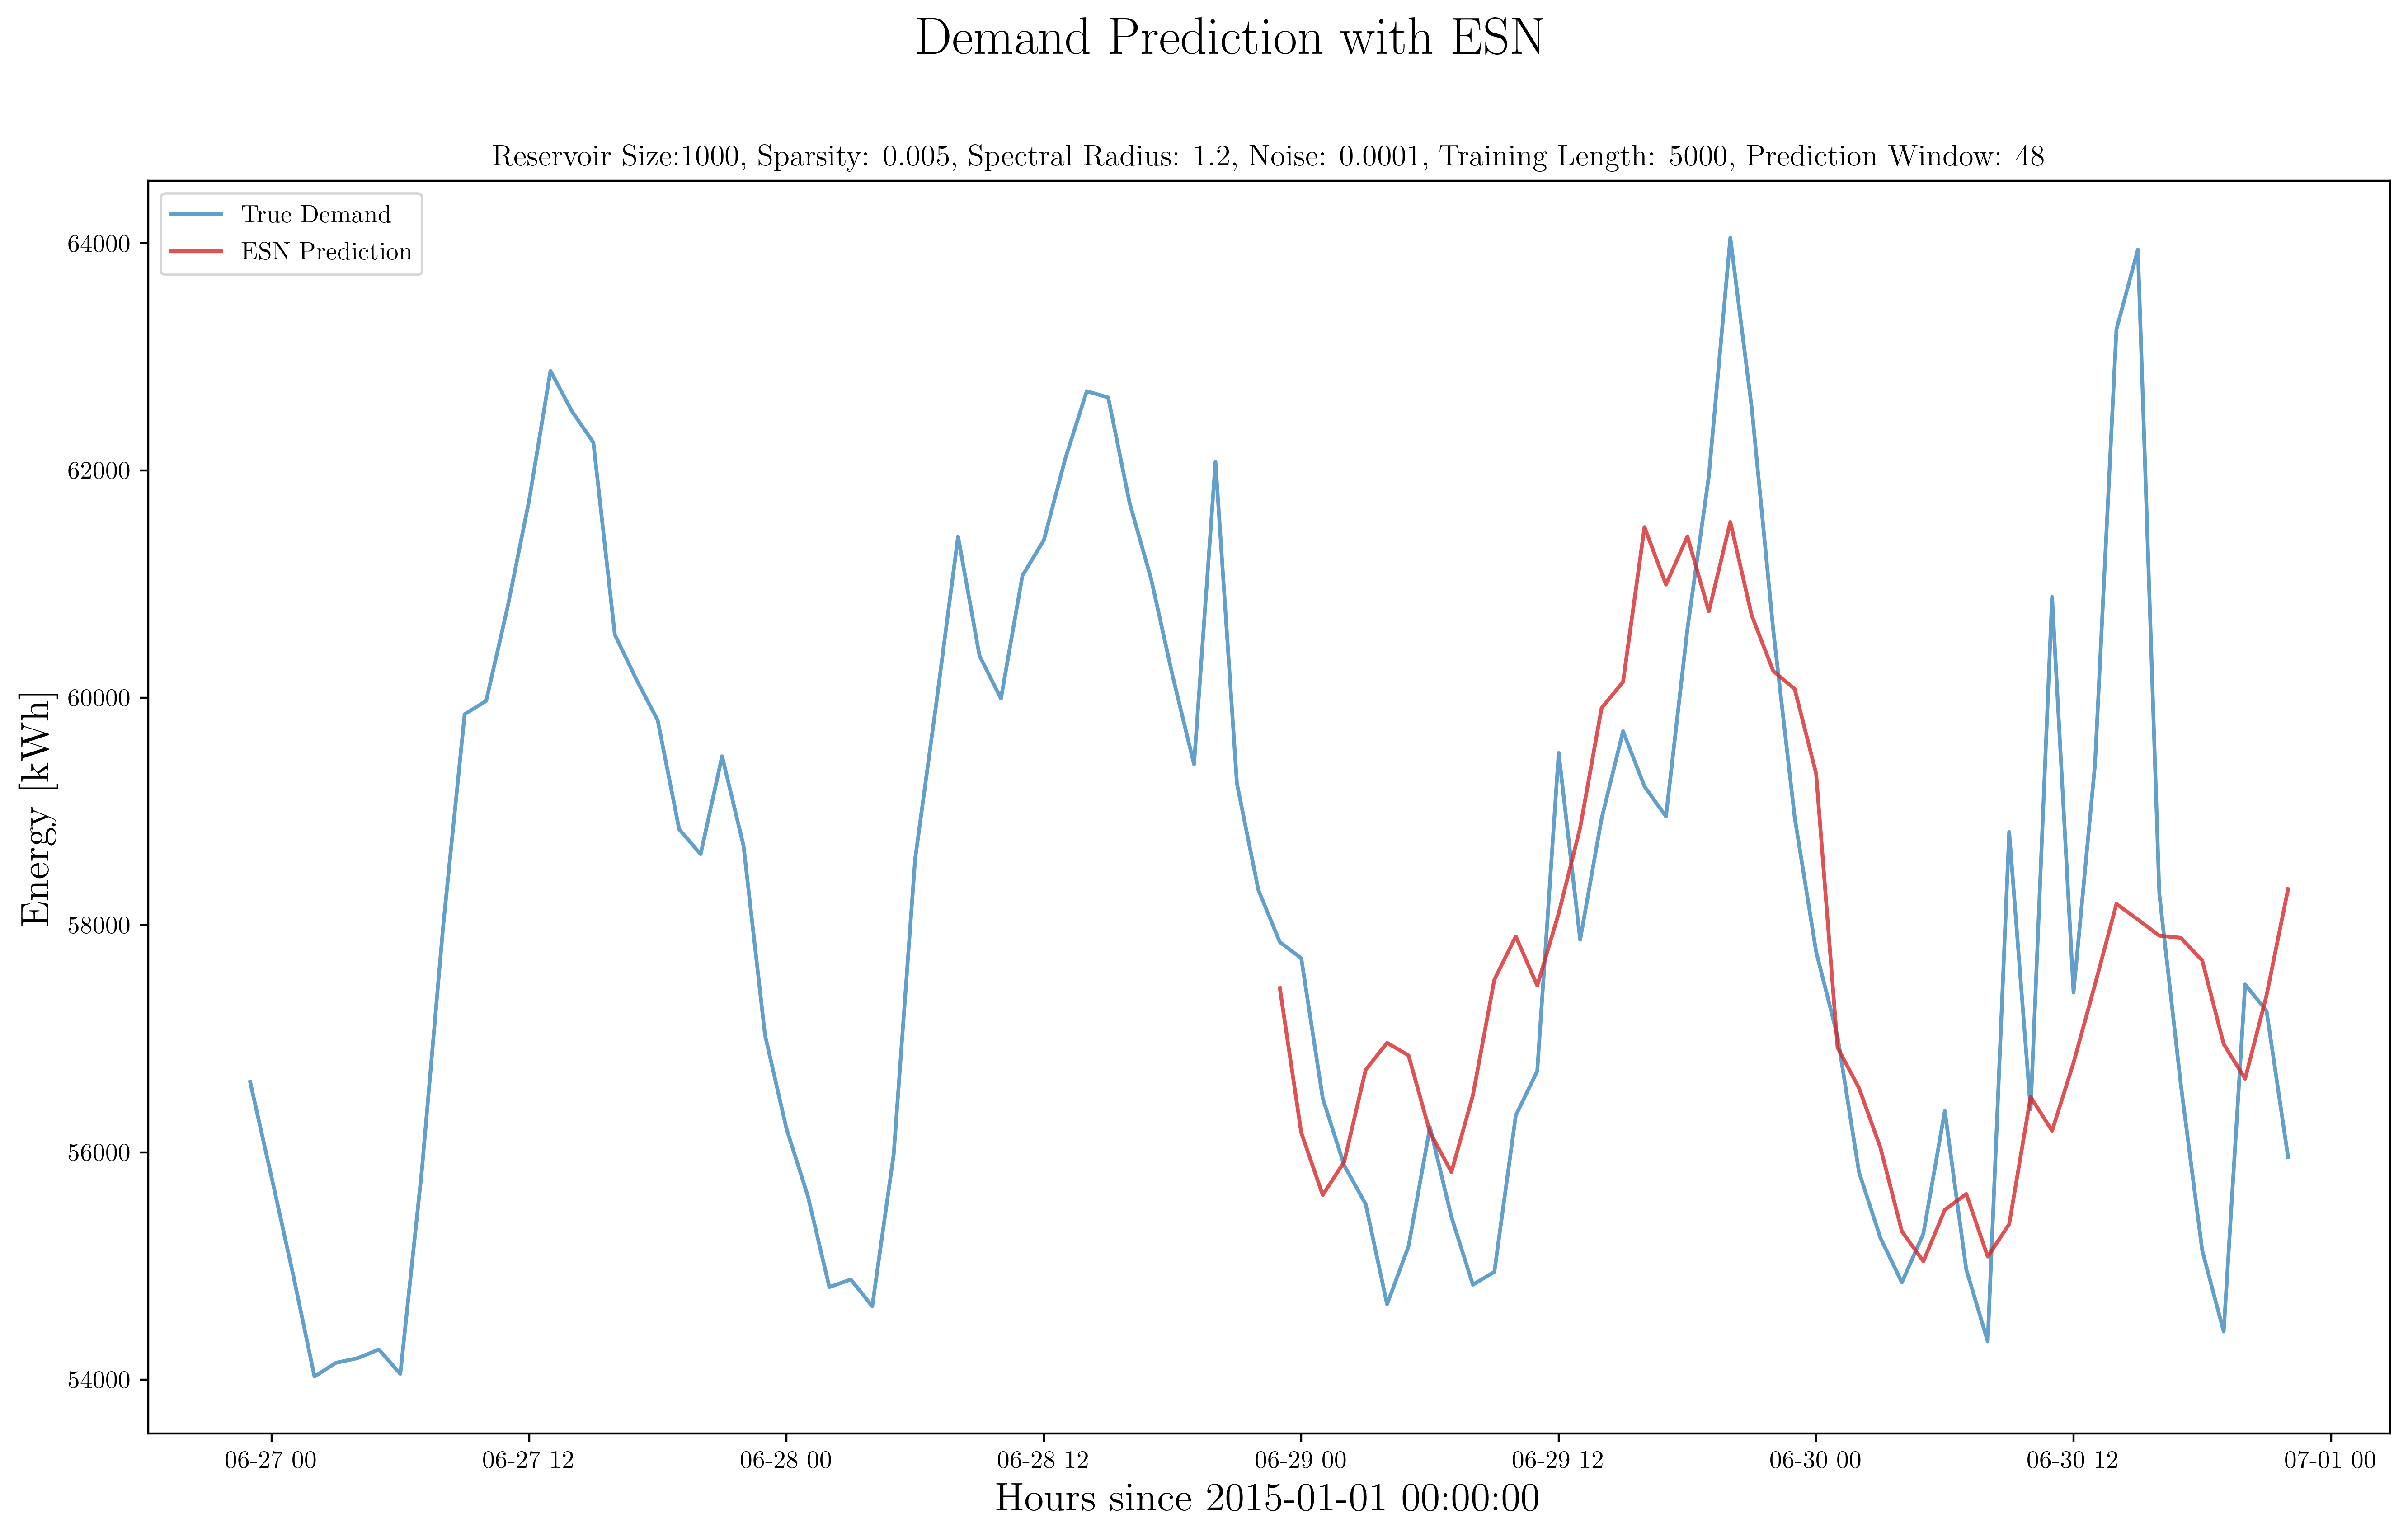
\includegraphics[width=0.8\textwidth]{48_demand_pressure_prediction.png}
  %% Creator: Matplotlib, PGF backend
%%
%% To include the figure in your LaTeX document, write
%%   \input{<filename>.pgf}
%%
%% Make sure the required packages are loaded in your preamble
%%   \usepackage{pgf}
%%
%% Figures using additional raster images can only be included by \input if
%% they are in the same directory as the main LaTeX file. For loading figures
%% from other directories you can use the `import` package
%%   \usepackage{import}
%% and then include the figures with
%%   \import{<path to file>}{<filename>.pgf}
%%
%% Matplotlib used the following preamble
%%
\begingroup%
\makeatletter%
\begin{pgfpicture}%
\pgfpathrectangle{\pgfpointorigin}{\pgfqpoint{5.601141in}{3.164528in}}%
\pgfusepath{use as bounding box, clip}%
\begin{pgfscope}%
\pgfsetbuttcap%
\pgfsetmiterjoin%
\definecolor{currentfill}{rgb}{1.000000,1.000000,1.000000}%
\pgfsetfillcolor{currentfill}%
\pgfsetlinewidth{0.000000pt}%
\definecolor{currentstroke}{rgb}{1.000000,1.000000,1.000000}%
\pgfsetstrokecolor{currentstroke}%
\pgfsetdash{}{0pt}%
\pgfpathmoveto{\pgfqpoint{0.000000in}{0.000000in}}%
\pgfpathlineto{\pgfqpoint{5.601141in}{0.000000in}}%
\pgfpathlineto{\pgfqpoint{5.601141in}{3.164528in}}%
\pgfpathlineto{\pgfqpoint{0.000000in}{3.164528in}}%
\pgfpathclose%
\pgfusepath{fill}%
\end{pgfscope}%
\begin{pgfscope}%
\pgfsetbuttcap%
\pgfsetmiterjoin%
\definecolor{currentfill}{rgb}{1.000000,1.000000,1.000000}%
\pgfsetfillcolor{currentfill}%
\pgfsetlinewidth{0.000000pt}%
\definecolor{currentstroke}{rgb}{0.000000,0.000000,0.000000}%
\pgfsetstrokecolor{currentstroke}%
\pgfsetstrokeopacity{0.000000}%
\pgfsetdash{}{0pt}%
\pgfpathmoveto{\pgfqpoint{0.738890in}{0.499691in}}%
\pgfpathlineto{\pgfqpoint{5.501141in}{0.499691in}}%
\pgfpathlineto{\pgfqpoint{5.501141in}{2.865455in}}%
\pgfpathlineto{\pgfqpoint{0.738890in}{2.865455in}}%
\pgfpathclose%
\pgfusepath{fill}%
\end{pgfscope}%
\begin{pgfscope}%
\pgfsetbuttcap%
\pgfsetroundjoin%
\definecolor{currentfill}{rgb}{0.000000,0.000000,0.000000}%
\pgfsetfillcolor{currentfill}%
\pgfsetlinewidth{0.803000pt}%
\definecolor{currentstroke}{rgb}{0.000000,0.000000,0.000000}%
\pgfsetstrokecolor{currentstroke}%
\pgfsetdash{}{0pt}%
\pgfsys@defobject{currentmarker}{\pgfqpoint{0.000000in}{-0.048611in}}{\pgfqpoint{0.000000in}{0.000000in}}{%
\pgfpathmoveto{\pgfqpoint{0.000000in}{0.000000in}}%
\pgfpathlineto{\pgfqpoint{0.000000in}{-0.048611in}}%
\pgfusepath{stroke,fill}%
}%
\begin{pgfscope}%
\pgfsys@transformshift{1.365502in}{0.499691in}%
\pgfsys@useobject{currentmarker}{}%
\end{pgfscope}%
\end{pgfscope}%
\begin{pgfscope}%
\definecolor{textcolor}{rgb}{0.000000,0.000000,0.000000}%
\pgfsetstrokecolor{textcolor}%
\pgfsetfillcolor{textcolor}%
\pgftext[x=1.365502in,y=0.402469in,,top]{\color{textcolor}\rmfamily\fontsize{10.000000}{12.000000}\selectfont \(\displaystyle 39320\)}%
\end{pgfscope}%
\begin{pgfscope}%
\pgfsetbuttcap%
\pgfsetroundjoin%
\definecolor{currentfill}{rgb}{0.000000,0.000000,0.000000}%
\pgfsetfillcolor{currentfill}%
\pgfsetlinewidth{0.803000pt}%
\definecolor{currentstroke}{rgb}{0.000000,0.000000,0.000000}%
\pgfsetstrokecolor{currentstroke}%
\pgfsetdash{}{0pt}%
\pgfsys@defobject{currentmarker}{\pgfqpoint{0.000000in}{-0.048611in}}{\pgfqpoint{0.000000in}{0.000000in}}{%
\pgfpathmoveto{\pgfqpoint{0.000000in}{0.000000in}}%
\pgfpathlineto{\pgfqpoint{0.000000in}{-0.048611in}}%
\pgfusepath{stroke,fill}%
}%
\begin{pgfscope}%
\pgfsys@transformshift{2.276938in}{0.499691in}%
\pgfsys@useobject{currentmarker}{}%
\end{pgfscope}%
\end{pgfscope}%
\begin{pgfscope}%
\definecolor{textcolor}{rgb}{0.000000,0.000000,0.000000}%
\pgfsetstrokecolor{textcolor}%
\pgfsetfillcolor{textcolor}%
\pgftext[x=2.276938in,y=0.402469in,,top]{\color{textcolor}\rmfamily\fontsize{10.000000}{12.000000}\selectfont \(\displaystyle 39340\)}%
\end{pgfscope}%
\begin{pgfscope}%
\pgfsetbuttcap%
\pgfsetroundjoin%
\definecolor{currentfill}{rgb}{0.000000,0.000000,0.000000}%
\pgfsetfillcolor{currentfill}%
\pgfsetlinewidth{0.803000pt}%
\definecolor{currentstroke}{rgb}{0.000000,0.000000,0.000000}%
\pgfsetstrokecolor{currentstroke}%
\pgfsetdash{}{0pt}%
\pgfsys@defobject{currentmarker}{\pgfqpoint{0.000000in}{-0.048611in}}{\pgfqpoint{0.000000in}{0.000000in}}{%
\pgfpathmoveto{\pgfqpoint{0.000000in}{0.000000in}}%
\pgfpathlineto{\pgfqpoint{0.000000in}{-0.048611in}}%
\pgfusepath{stroke,fill}%
}%
\begin{pgfscope}%
\pgfsys@transformshift{3.188373in}{0.499691in}%
\pgfsys@useobject{currentmarker}{}%
\end{pgfscope}%
\end{pgfscope}%
\begin{pgfscope}%
\definecolor{textcolor}{rgb}{0.000000,0.000000,0.000000}%
\pgfsetstrokecolor{textcolor}%
\pgfsetfillcolor{textcolor}%
\pgftext[x=3.188373in,y=0.402469in,,top]{\color{textcolor}\rmfamily\fontsize{10.000000}{12.000000}\selectfont \(\displaystyle 39360\)}%
\end{pgfscope}%
\begin{pgfscope}%
\pgfsetbuttcap%
\pgfsetroundjoin%
\definecolor{currentfill}{rgb}{0.000000,0.000000,0.000000}%
\pgfsetfillcolor{currentfill}%
\pgfsetlinewidth{0.803000pt}%
\definecolor{currentstroke}{rgb}{0.000000,0.000000,0.000000}%
\pgfsetstrokecolor{currentstroke}%
\pgfsetdash{}{0pt}%
\pgfsys@defobject{currentmarker}{\pgfqpoint{0.000000in}{-0.048611in}}{\pgfqpoint{0.000000in}{0.000000in}}{%
\pgfpathmoveto{\pgfqpoint{0.000000in}{0.000000in}}%
\pgfpathlineto{\pgfqpoint{0.000000in}{-0.048611in}}%
\pgfusepath{stroke,fill}%
}%
\begin{pgfscope}%
\pgfsys@transformshift{4.099809in}{0.499691in}%
\pgfsys@useobject{currentmarker}{}%
\end{pgfscope}%
\end{pgfscope}%
\begin{pgfscope}%
\definecolor{textcolor}{rgb}{0.000000,0.000000,0.000000}%
\pgfsetstrokecolor{textcolor}%
\pgfsetfillcolor{textcolor}%
\pgftext[x=4.099809in,y=0.402469in,,top]{\color{textcolor}\rmfamily\fontsize{10.000000}{12.000000}\selectfont \(\displaystyle 39380\)}%
\end{pgfscope}%
\begin{pgfscope}%
\pgfsetbuttcap%
\pgfsetroundjoin%
\definecolor{currentfill}{rgb}{0.000000,0.000000,0.000000}%
\pgfsetfillcolor{currentfill}%
\pgfsetlinewidth{0.803000pt}%
\definecolor{currentstroke}{rgb}{0.000000,0.000000,0.000000}%
\pgfsetstrokecolor{currentstroke}%
\pgfsetdash{}{0pt}%
\pgfsys@defobject{currentmarker}{\pgfqpoint{0.000000in}{-0.048611in}}{\pgfqpoint{0.000000in}{0.000000in}}{%
\pgfpathmoveto{\pgfqpoint{0.000000in}{0.000000in}}%
\pgfpathlineto{\pgfqpoint{0.000000in}{-0.048611in}}%
\pgfusepath{stroke,fill}%
}%
\begin{pgfscope}%
\pgfsys@transformshift{5.011244in}{0.499691in}%
\pgfsys@useobject{currentmarker}{}%
\end{pgfscope}%
\end{pgfscope}%
\begin{pgfscope}%
\definecolor{textcolor}{rgb}{0.000000,0.000000,0.000000}%
\pgfsetstrokecolor{textcolor}%
\pgfsetfillcolor{textcolor}%
\pgftext[x=5.011244in,y=0.402469in,,top]{\color{textcolor}\rmfamily\fontsize{10.000000}{12.000000}\selectfont \(\displaystyle 39400\)}%
\end{pgfscope}%
\begin{pgfscope}%
\definecolor{textcolor}{rgb}{0.000000,0.000000,0.000000}%
\pgfsetstrokecolor{textcolor}%
\pgfsetfillcolor{textcolor}%
\pgftext[x=3.120016in,y=0.223457in,,top]{\color{textcolor}\rmfamily\fontsize{10.000000}{12.000000}\selectfont Hours since 2015-01-01 00:00:00}%
\end{pgfscope}%
\begin{pgfscope}%
\pgfsetbuttcap%
\pgfsetroundjoin%
\definecolor{currentfill}{rgb}{0.000000,0.000000,0.000000}%
\pgfsetfillcolor{currentfill}%
\pgfsetlinewidth{0.803000pt}%
\definecolor{currentstroke}{rgb}{0.000000,0.000000,0.000000}%
\pgfsetstrokecolor{currentstroke}%
\pgfsetdash{}{0pt}%
\pgfsys@defobject{currentmarker}{\pgfqpoint{-0.048611in}{0.000000in}}{\pgfqpoint{0.000000in}{0.000000in}}{%
\pgfpathmoveto{\pgfqpoint{0.000000in}{0.000000in}}%
\pgfpathlineto{\pgfqpoint{-0.048611in}{0.000000in}}%
\pgfusepath{stroke,fill}%
}%
\begin{pgfscope}%
\pgfsys@transformshift{0.738890in}{0.610376in}%
\pgfsys@useobject{currentmarker}{}%
\end{pgfscope}%
\end{pgfscope}%
\begin{pgfscope}%
\definecolor{textcolor}{rgb}{0.000000,0.000000,0.000000}%
\pgfsetstrokecolor{textcolor}%
\pgfsetfillcolor{textcolor}%
\pgftext[x=0.294444in,y=0.562150in,left,base]{\color{textcolor}\rmfamily\fontsize{10.000000}{12.000000}\selectfont \(\displaystyle 54000\)}%
\end{pgfscope}%
\begin{pgfscope}%
\pgfsetbuttcap%
\pgfsetroundjoin%
\definecolor{currentfill}{rgb}{0.000000,0.000000,0.000000}%
\pgfsetfillcolor{currentfill}%
\pgfsetlinewidth{0.803000pt}%
\definecolor{currentstroke}{rgb}{0.000000,0.000000,0.000000}%
\pgfsetstrokecolor{currentstroke}%
\pgfsetdash{}{0pt}%
\pgfsys@defobject{currentmarker}{\pgfqpoint{-0.048611in}{0.000000in}}{\pgfqpoint{0.000000in}{0.000000in}}{%
\pgfpathmoveto{\pgfqpoint{0.000000in}{0.000000in}}%
\pgfpathlineto{\pgfqpoint{-0.048611in}{0.000000in}}%
\pgfusepath{stroke,fill}%
}%
\begin{pgfscope}%
\pgfsys@transformshift{0.738890in}{1.037790in}%
\pgfsys@useobject{currentmarker}{}%
\end{pgfscope}%
\end{pgfscope}%
\begin{pgfscope}%
\definecolor{textcolor}{rgb}{0.000000,0.000000,0.000000}%
\pgfsetstrokecolor{textcolor}%
\pgfsetfillcolor{textcolor}%
\pgftext[x=0.294444in,y=0.989565in,left,base]{\color{textcolor}\rmfamily\fontsize{10.000000}{12.000000}\selectfont \(\displaystyle 56000\)}%
\end{pgfscope}%
\begin{pgfscope}%
\pgfsetbuttcap%
\pgfsetroundjoin%
\definecolor{currentfill}{rgb}{0.000000,0.000000,0.000000}%
\pgfsetfillcolor{currentfill}%
\pgfsetlinewidth{0.803000pt}%
\definecolor{currentstroke}{rgb}{0.000000,0.000000,0.000000}%
\pgfsetstrokecolor{currentstroke}%
\pgfsetdash{}{0pt}%
\pgfsys@defobject{currentmarker}{\pgfqpoint{-0.048611in}{0.000000in}}{\pgfqpoint{0.000000in}{0.000000in}}{%
\pgfpathmoveto{\pgfqpoint{0.000000in}{0.000000in}}%
\pgfpathlineto{\pgfqpoint{-0.048611in}{0.000000in}}%
\pgfusepath{stroke,fill}%
}%
\begin{pgfscope}%
\pgfsys@transformshift{0.738890in}{1.465205in}%
\pgfsys@useobject{currentmarker}{}%
\end{pgfscope}%
\end{pgfscope}%
\begin{pgfscope}%
\definecolor{textcolor}{rgb}{0.000000,0.000000,0.000000}%
\pgfsetstrokecolor{textcolor}%
\pgfsetfillcolor{textcolor}%
\pgftext[x=0.294444in,y=1.416979in,left,base]{\color{textcolor}\rmfamily\fontsize{10.000000}{12.000000}\selectfont \(\displaystyle 58000\)}%
\end{pgfscope}%
\begin{pgfscope}%
\pgfsetbuttcap%
\pgfsetroundjoin%
\definecolor{currentfill}{rgb}{0.000000,0.000000,0.000000}%
\pgfsetfillcolor{currentfill}%
\pgfsetlinewidth{0.803000pt}%
\definecolor{currentstroke}{rgb}{0.000000,0.000000,0.000000}%
\pgfsetstrokecolor{currentstroke}%
\pgfsetdash{}{0pt}%
\pgfsys@defobject{currentmarker}{\pgfqpoint{-0.048611in}{0.000000in}}{\pgfqpoint{0.000000in}{0.000000in}}{%
\pgfpathmoveto{\pgfqpoint{0.000000in}{0.000000in}}%
\pgfpathlineto{\pgfqpoint{-0.048611in}{0.000000in}}%
\pgfusepath{stroke,fill}%
}%
\begin{pgfscope}%
\pgfsys@transformshift{0.738890in}{1.892619in}%
\pgfsys@useobject{currentmarker}{}%
\end{pgfscope}%
\end{pgfscope}%
\begin{pgfscope}%
\definecolor{textcolor}{rgb}{0.000000,0.000000,0.000000}%
\pgfsetstrokecolor{textcolor}%
\pgfsetfillcolor{textcolor}%
\pgftext[x=0.294444in,y=1.844394in,left,base]{\color{textcolor}\rmfamily\fontsize{10.000000}{12.000000}\selectfont \(\displaystyle 60000\)}%
\end{pgfscope}%
\begin{pgfscope}%
\pgfsetbuttcap%
\pgfsetroundjoin%
\definecolor{currentfill}{rgb}{0.000000,0.000000,0.000000}%
\pgfsetfillcolor{currentfill}%
\pgfsetlinewidth{0.803000pt}%
\definecolor{currentstroke}{rgb}{0.000000,0.000000,0.000000}%
\pgfsetstrokecolor{currentstroke}%
\pgfsetdash{}{0pt}%
\pgfsys@defobject{currentmarker}{\pgfqpoint{-0.048611in}{0.000000in}}{\pgfqpoint{0.000000in}{0.000000in}}{%
\pgfpathmoveto{\pgfqpoint{0.000000in}{0.000000in}}%
\pgfpathlineto{\pgfqpoint{-0.048611in}{0.000000in}}%
\pgfusepath{stroke,fill}%
}%
\begin{pgfscope}%
\pgfsys@transformshift{0.738890in}{2.320034in}%
\pgfsys@useobject{currentmarker}{}%
\end{pgfscope}%
\end{pgfscope}%
\begin{pgfscope}%
\definecolor{textcolor}{rgb}{0.000000,0.000000,0.000000}%
\pgfsetstrokecolor{textcolor}%
\pgfsetfillcolor{textcolor}%
\pgftext[x=0.294444in,y=2.271808in,left,base]{\color{textcolor}\rmfamily\fontsize{10.000000}{12.000000}\selectfont \(\displaystyle 62000\)}%
\end{pgfscope}%
\begin{pgfscope}%
\pgfsetbuttcap%
\pgfsetroundjoin%
\definecolor{currentfill}{rgb}{0.000000,0.000000,0.000000}%
\pgfsetfillcolor{currentfill}%
\pgfsetlinewidth{0.803000pt}%
\definecolor{currentstroke}{rgb}{0.000000,0.000000,0.000000}%
\pgfsetstrokecolor{currentstroke}%
\pgfsetdash{}{0pt}%
\pgfsys@defobject{currentmarker}{\pgfqpoint{-0.048611in}{0.000000in}}{\pgfqpoint{0.000000in}{0.000000in}}{%
\pgfpathmoveto{\pgfqpoint{0.000000in}{0.000000in}}%
\pgfpathlineto{\pgfqpoint{-0.048611in}{0.000000in}}%
\pgfusepath{stroke,fill}%
}%
\begin{pgfscope}%
\pgfsys@transformshift{0.738890in}{2.747448in}%
\pgfsys@useobject{currentmarker}{}%
\end{pgfscope}%
\end{pgfscope}%
\begin{pgfscope}%
\definecolor{textcolor}{rgb}{0.000000,0.000000,0.000000}%
\pgfsetstrokecolor{textcolor}%
\pgfsetfillcolor{textcolor}%
\pgftext[x=0.294444in,y=2.699223in,left,base]{\color{textcolor}\rmfamily\fontsize{10.000000}{12.000000}\selectfont \(\displaystyle 64000\)}%
\end{pgfscope}%
\begin{pgfscope}%
\definecolor{textcolor}{rgb}{0.000000,0.000000,0.000000}%
\pgfsetstrokecolor{textcolor}%
\pgfsetfillcolor{textcolor}%
\pgftext[x=0.238889in,y=1.682573in,,bottom,rotate=90.000000]{\color{textcolor}\rmfamily\fontsize{10.000000}{12.000000}\selectfont Energy [kWh]}%
\end{pgfscope}%
\begin{pgfscope}%
\pgfpathrectangle{\pgfqpoint{0.738890in}{0.499691in}}{\pgfqpoint{4.762251in}{2.365763in}}%
\pgfusepath{clip}%
\pgfsetrectcap%
\pgfsetroundjoin%
\pgfsetlinewidth{1.505625pt}%
\definecolor{currentstroke}{rgb}{0.121569,0.466667,0.705882}%
\pgfsetstrokecolor{currentstroke}%
\pgfsetstrokeopacity{0.700000}%
\pgfsetdash{}{0pt}%
\pgfpathmoveto{\pgfqpoint{0.955356in}{1.170289in}}%
\pgfpathlineto{\pgfqpoint{1.000928in}{0.990774in}}%
\pgfpathlineto{\pgfqpoint{1.046500in}{0.808482in}}%
\pgfpathlineto{\pgfqpoint{1.092071in}{0.616146in}}%
\pgfpathlineto{\pgfqpoint{1.137643in}{0.642004in}}%
\pgfpathlineto{\pgfqpoint{1.183215in}{0.650553in}}%
\pgfpathlineto{\pgfqpoint{1.228787in}{0.667008in}}%
\pgfpathlineto{\pgfqpoint{1.274358in}{0.621061in}}%
\pgfpathlineto{\pgfqpoint{1.319930in}{1.002101in}}%
\pgfpathlineto{\pgfqpoint{1.365502in}{1.464136in}}%
\pgfpathlineto{\pgfqpoint{1.411074in}{1.861845in}}%
\pgfpathlineto{\pgfqpoint{1.456646in}{1.886635in}}%
\pgfpathlineto{\pgfqpoint{1.502217in}{2.062944in}}%
\pgfpathlineto{\pgfqpoint{1.547789in}{2.262760in}}%
\pgfpathlineto{\pgfqpoint{1.593361in}{2.507455in}}%
\pgfpathlineto{\pgfqpoint{1.638933in}{2.431589in}}%
\pgfpathlineto{\pgfqpoint{1.684504in}{2.372819in}}%
\pgfpathlineto{\pgfqpoint{1.730076in}{2.011440in}}%
\pgfpathlineto{\pgfqpoint{1.775648in}{1.927453in}}%
\pgfpathlineto{\pgfqpoint{1.821220in}{1.850091in}}%
\pgfpathlineto{\pgfqpoint{1.866792in}{1.645360in}}%
\pgfpathlineto{\pgfqpoint{1.912363in}{1.598558in}}%
\pgfpathlineto{\pgfqpoint{1.957935in}{1.782774in}}%
\pgfpathlineto{\pgfqpoint{2.003507in}{1.614372in}}%
\pgfpathlineto{\pgfqpoint{2.049079in}{1.258763in}}%
\pgfpathlineto{\pgfqpoint{2.094650in}{1.082455in}}%
\pgfpathlineto{\pgfqpoint{2.140222in}{0.955299in}}%
\pgfpathlineto{\pgfqpoint{2.185794in}{0.784333in}}%
\pgfpathlineto{\pgfqpoint{2.231366in}{0.798652in}}%
\pgfpathlineto{\pgfqpoint{2.276938in}{0.748217in}}%
\pgfpathlineto{\pgfqpoint{2.322509in}{1.034157in}}%
\pgfpathlineto{\pgfqpoint{2.368081in}{1.589369in}}%
\pgfpathlineto{\pgfqpoint{2.413653in}{1.886635in}}%
\pgfpathlineto{\pgfqpoint{2.459225in}{2.196083in}}%
\pgfpathlineto{\pgfqpoint{2.504796in}{1.971691in}}%
\pgfpathlineto{\pgfqpoint{2.550368in}{1.891123in}}%
\pgfpathlineto{\pgfqpoint{2.595940in}{2.122141in}}%
\pgfpathlineto{\pgfqpoint{2.641512in}{2.189245in}}%
\pgfpathlineto{\pgfqpoint{2.687084in}{2.342687in}}%
\pgfpathlineto{\pgfqpoint{2.732655in}{2.469201in}}%
\pgfpathlineto{\pgfqpoint{2.778227in}{2.457447in}}%
\pgfpathlineto{\pgfqpoint{2.823799in}{2.258700in}}%
\pgfpathlineto{\pgfqpoint{2.869371in}{2.116371in}}%
\pgfpathlineto{\pgfqpoint{2.914942in}{1.934292in}}%
\pgfpathlineto{\pgfqpoint{2.960514in}{1.767600in}}%
\pgfpathlineto{\pgfqpoint{3.006086in}{2.336703in}}%
\pgfpathlineto{\pgfqpoint{3.051658in}{1.731484in}}%
\pgfpathlineto{\pgfqpoint{3.097230in}{1.531240in}}%
\pgfpathlineto{\pgfqpoint{3.142801in}{1.433149in}}%
\pgfpathlineto{\pgfqpoint{3.188373in}{1.402802in}}%
\pgfpathlineto{\pgfqpoint{3.233945in}{1.139515in}}%
\pgfpathlineto{\pgfqpoint{3.279517in}{1.013214in}}%
\pgfpathlineto{\pgfqpoint{3.325089in}{0.940553in}}%
\pgfpathlineto{\pgfqpoint{3.370660in}{0.752063in}}%
\pgfpathlineto{\pgfqpoint{3.416232in}{0.861268in}}%
\pgfpathlineto{\pgfqpoint{3.461804in}{1.085233in}}%
\pgfpathlineto{\pgfqpoint{3.507376in}{0.916191in}}%
\pgfpathlineto{\pgfqpoint{3.552947in}{0.788821in}}%
\pgfpathlineto{\pgfqpoint{3.598519in}{0.812970in}}%
\pgfpathlineto{\pgfqpoint{3.644091in}{1.107245in}}%
\pgfpathlineto{\pgfqpoint{3.689663in}{1.190591in}}%
\pgfpathlineto{\pgfqpoint{3.735235in}{1.788971in}}%
\pgfpathlineto{\pgfqpoint{3.780806in}{1.437636in}}%
\pgfpathlineto{\pgfqpoint{3.826378in}{1.665448in}}%
\pgfpathlineto{\pgfqpoint{3.871950in}{1.829789in}}%
\pgfpathlineto{\pgfqpoint{3.917522in}{1.725927in}}%
\pgfpathlineto{\pgfqpoint{3.963093in}{1.669509in}}%
\pgfpathlineto{\pgfqpoint{4.008665in}{2.021912in}}%
\pgfpathlineto{\pgfqpoint{4.054237in}{2.309989in}}%
\pgfpathlineto{\pgfqpoint{4.099809in}{2.757920in}}%
\pgfpathlineto{\pgfqpoint{4.145381in}{2.437573in}}%
\pgfpathlineto{\pgfqpoint{4.190952in}{2.021057in}}%
\pgfpathlineto{\pgfqpoint{4.236524in}{1.668227in}}%
\pgfpathlineto{\pgfqpoint{4.282096in}{1.415411in}}%
\pgfpathlineto{\pgfqpoint{4.327668in}{1.255771in}}%
\pgfpathlineto{\pgfqpoint{4.373239in}{1.000391in}}%
\pgfpathlineto{\pgfqpoint{4.418811in}{0.876655in}}%
\pgfpathlineto{\pgfqpoint{4.464383in}{0.793095in}}%
\pgfpathlineto{\pgfqpoint{4.509955in}{0.884989in}}%
\pgfpathlineto{\pgfqpoint{4.555527in}{1.115580in}}%
\pgfpathlineto{\pgfqpoint{4.601098in}{0.817458in}}%
\pgfpathlineto{\pgfqpoint{4.646670in}{0.682181in}}%
\pgfpathlineto{\pgfqpoint{4.692242in}{1.640658in}}%
\pgfpathlineto{\pgfqpoint{4.737814in}{1.118358in}}%
\pgfpathlineto{\pgfqpoint{4.783385in}{2.082605in}}%
\pgfpathlineto{\pgfqpoint{4.828957in}{1.338476in}}%
\pgfpathlineto{\pgfqpoint{4.874529in}{1.767173in}}%
\pgfpathlineto{\pgfqpoint{4.920101in}{2.585458in}}%
\pgfpathlineto{\pgfqpoint{4.965673in}{2.735694in}}%
\pgfpathlineto{\pgfqpoint{5.011244in}{1.523333in}}%
\pgfpathlineto{\pgfqpoint{5.056816in}{1.165801in}}%
\pgfpathlineto{\pgfqpoint{5.102388in}{0.853147in}}%
\pgfpathlineto{\pgfqpoint{5.147960in}{0.700774in}}%
\pgfpathlineto{\pgfqpoint{5.193531in}{1.353649in}}%
\pgfpathlineto{\pgfqpoint{5.239103in}{1.303428in}}%
\pgfpathlineto{\pgfqpoint{5.284675in}{1.029028in}}%
\pgfusepath{stroke}%
\end{pgfscope}%
\begin{pgfscope}%
\pgfpathrectangle{\pgfqpoint{0.738890in}{0.499691in}}{\pgfqpoint{4.762251in}{2.365763in}}%
\pgfusepath{clip}%
\pgfsetrectcap%
\pgfsetroundjoin%
\pgfsetlinewidth{1.505625pt}%
\definecolor{currentstroke}{rgb}{0.839216,0.152941,0.156863}%
\pgfsetstrokecolor{currentstroke}%
\pgfsetstrokeopacity{0.800000}%
\pgfsetdash{}{0pt}%
\pgfpathmoveto{\pgfqpoint{3.142801in}{1.499160in}}%
\pgfpathlineto{\pgfqpoint{3.188373in}{1.729002in}}%
\pgfpathlineto{\pgfqpoint{3.233945in}{1.184696in}}%
\pgfpathlineto{\pgfqpoint{3.279517in}{1.134258in}}%
\pgfpathlineto{\pgfqpoint{3.325089in}{0.902954in}}%
\pgfpathlineto{\pgfqpoint{3.370660in}{0.820833in}}%
\pgfpathlineto{\pgfqpoint{3.416232in}{0.607226in}}%
\pgfpathlineto{\pgfqpoint{3.461804in}{0.989923in}}%
\pgfpathlineto{\pgfqpoint{3.507376in}{1.170307in}}%
\pgfpathlineto{\pgfqpoint{3.552947in}{1.573560in}}%
\pgfpathlineto{\pgfqpoint{3.598519in}{1.717692in}}%
\pgfpathlineto{\pgfqpoint{3.644091in}{1.931528in}}%
\pgfpathlineto{\pgfqpoint{3.689663in}{1.740147in}}%
\pgfpathlineto{\pgfqpoint{3.735235in}{2.103523in}}%
\pgfpathlineto{\pgfqpoint{3.780806in}{1.952481in}}%
\pgfpathlineto{\pgfqpoint{3.826378in}{2.262303in}}%
\pgfpathlineto{\pgfqpoint{3.871950in}{2.031406in}}%
\pgfpathlineto{\pgfqpoint{3.917522in}{1.940224in}}%
\pgfpathlineto{\pgfqpoint{3.963093in}{1.588777in}}%
\pgfpathlineto{\pgfqpoint{4.008665in}{1.818859in}}%
\pgfpathlineto{\pgfqpoint{4.054237in}{1.834700in}}%
\pgfpathlineto{\pgfqpoint{4.099809in}{2.191688in}}%
\pgfpathlineto{\pgfqpoint{4.145381in}{1.914665in}}%
\pgfpathlineto{\pgfqpoint{4.190952in}{1.822193in}}%
\pgfpathlineto{\pgfqpoint{4.236524in}{1.576811in}}%
\pgfpathlineto{\pgfqpoint{4.282096in}{1.635439in}}%
\pgfpathlineto{\pgfqpoint{4.327668in}{1.213959in}}%
\pgfpathlineto{\pgfqpoint{4.373239in}{1.113797in}}%
\pgfpathlineto{\pgfqpoint{4.418811in}{1.111707in}}%
\pgfpathlineto{\pgfqpoint{4.464383in}{1.024680in}}%
\pgfpathlineto{\pgfqpoint{4.509955in}{0.982283in}}%
\pgfpathlineto{\pgfqpoint{4.555527in}{1.329969in}}%
\pgfpathlineto{\pgfqpoint{4.601098in}{1.137540in}}%
\pgfpathlineto{\pgfqpoint{4.646670in}{1.376801in}}%
\pgfpathlineto{\pgfqpoint{4.692242in}{1.347719in}}%
\pgfpathlineto{\pgfqpoint{4.737814in}{1.545751in}}%
\pgfpathlineto{\pgfqpoint{4.783385in}{1.662906in}}%
\pgfpathlineto{\pgfqpoint{4.828957in}{1.614829in}}%
\pgfpathlineto{\pgfqpoint{4.874529in}{1.882985in}}%
\pgfpathlineto{\pgfqpoint{4.920101in}{2.036722in}}%
\pgfpathlineto{\pgfqpoint{4.965673in}{1.912560in}}%
\pgfpathlineto{\pgfqpoint{5.011244in}{1.711386in}}%
\pgfpathlineto{\pgfqpoint{5.056816in}{1.530486in}}%
\pgfpathlineto{\pgfqpoint{5.102388in}{1.120176in}}%
\pgfpathlineto{\pgfqpoint{5.147960in}{1.095955in}}%
\pgfpathlineto{\pgfqpoint{5.193531in}{1.320882in}}%
\pgfpathlineto{\pgfqpoint{5.239103in}{1.493131in}}%
\pgfpathlineto{\pgfqpoint{5.284675in}{1.310791in}}%
\pgfusepath{stroke}%
\end{pgfscope}%
\begin{pgfscope}%
\pgfsetrectcap%
\pgfsetmiterjoin%
\pgfsetlinewidth{0.803000pt}%
\definecolor{currentstroke}{rgb}{0.000000,0.000000,0.000000}%
\pgfsetstrokecolor{currentstroke}%
\pgfsetdash{}{0pt}%
\pgfpathmoveto{\pgfqpoint{0.738890in}{0.499691in}}%
\pgfpathlineto{\pgfqpoint{0.738890in}{2.865455in}}%
\pgfusepath{stroke}%
\end{pgfscope}%
\begin{pgfscope}%
\pgfsetrectcap%
\pgfsetmiterjoin%
\pgfsetlinewidth{0.803000pt}%
\definecolor{currentstroke}{rgb}{0.000000,0.000000,0.000000}%
\pgfsetstrokecolor{currentstroke}%
\pgfsetdash{}{0pt}%
\pgfpathmoveto{\pgfqpoint{5.501141in}{0.499691in}}%
\pgfpathlineto{\pgfqpoint{5.501141in}{2.865455in}}%
\pgfusepath{stroke}%
\end{pgfscope}%
\begin{pgfscope}%
\pgfsetrectcap%
\pgfsetmiterjoin%
\pgfsetlinewidth{0.803000pt}%
\definecolor{currentstroke}{rgb}{0.000000,0.000000,0.000000}%
\pgfsetstrokecolor{currentstroke}%
\pgfsetdash{}{0pt}%
\pgfpathmoveto{\pgfqpoint{0.738890in}{0.499691in}}%
\pgfpathlineto{\pgfqpoint{5.501141in}{0.499691in}}%
\pgfusepath{stroke}%
\end{pgfscope}%
\begin{pgfscope}%
\pgfsetrectcap%
\pgfsetmiterjoin%
\pgfsetlinewidth{0.803000pt}%
\definecolor{currentstroke}{rgb}{0.000000,0.000000,0.000000}%
\pgfsetstrokecolor{currentstroke}%
\pgfsetdash{}{0pt}%
\pgfpathmoveto{\pgfqpoint{0.738890in}{2.865455in}}%
\pgfpathlineto{\pgfqpoint{5.501141in}{2.865455in}}%
\pgfusepath{stroke}%
\end{pgfscope}%
\begin{pgfscope}%
\definecolor{textcolor}{rgb}{0.000000,0.000000,0.000000}%
\pgfsetstrokecolor{textcolor}%
\pgfsetfillcolor{textcolor}%
\pgftext[x=3.120016in,y=2.948788in,,base]{\color{textcolor}\rmfamily\fontsize{12.000000}{14.400000}\selectfont Demand Prediction with an ESN}%
\end{pgfscope}%
\begin{pgfscope}%
\pgfsetbuttcap%
\pgfsetmiterjoin%
\definecolor{currentfill}{rgb}{1.000000,1.000000,1.000000}%
\pgfsetfillcolor{currentfill}%
\pgfsetfillopacity{0.800000}%
\pgfsetlinewidth{1.003750pt}%
\definecolor{currentstroke}{rgb}{0.800000,0.800000,0.800000}%
\pgfsetstrokecolor{currentstroke}%
\pgfsetstrokeopacity{0.800000}%
\pgfsetdash{}{0pt}%
\pgfpathmoveto{\pgfqpoint{0.836112in}{2.366998in}}%
\pgfpathlineto{\pgfqpoint{2.230018in}{2.366998in}}%
\pgfpathquadraticcurveto{\pgfqpoint{2.257796in}{2.366998in}}{\pgfqpoint{2.257796in}{2.394776in}}%
\pgfpathlineto{\pgfqpoint{2.257796in}{2.768232in}}%
\pgfpathquadraticcurveto{\pgfqpoint{2.257796in}{2.796010in}}{\pgfqpoint{2.230018in}{2.796010in}}%
\pgfpathlineto{\pgfqpoint{0.836112in}{2.796010in}}%
\pgfpathquadraticcurveto{\pgfqpoint{0.808334in}{2.796010in}}{\pgfqpoint{0.808334in}{2.768232in}}%
\pgfpathlineto{\pgfqpoint{0.808334in}{2.394776in}}%
\pgfpathquadraticcurveto{\pgfqpoint{0.808334in}{2.366998in}}{\pgfqpoint{0.836112in}{2.366998in}}%
\pgfpathclose%
\pgfusepath{stroke,fill}%
\end{pgfscope}%
\begin{pgfscope}%
\pgfsetrectcap%
\pgfsetroundjoin%
\pgfsetlinewidth{1.505625pt}%
\definecolor{currentstroke}{rgb}{0.121569,0.466667,0.705882}%
\pgfsetstrokecolor{currentstroke}%
\pgfsetstrokeopacity{0.700000}%
\pgfsetdash{}{0pt}%
\pgfpathmoveto{\pgfqpoint{0.863890in}{2.691843in}}%
\pgfpathlineto{\pgfqpoint{1.141668in}{2.691843in}}%
\pgfusepath{stroke}%
\end{pgfscope}%
\begin{pgfscope}%
\definecolor{textcolor}{rgb}{0.000000,0.000000,0.000000}%
\pgfsetstrokecolor{textcolor}%
\pgfsetfillcolor{textcolor}%
\pgftext[x=1.252779in,y=2.643232in,left,base]{\color{textcolor}\rmfamily\fontsize{10.000000}{12.000000}\selectfont True Demand}%
\end{pgfscope}%
\begin{pgfscope}%
\pgfsetrectcap%
\pgfsetroundjoin%
\pgfsetlinewidth{1.505625pt}%
\definecolor{currentstroke}{rgb}{0.839216,0.152941,0.156863}%
\pgfsetstrokecolor{currentstroke}%
\pgfsetstrokeopacity{0.800000}%
\pgfsetdash{}{0pt}%
\pgfpathmoveto{\pgfqpoint{0.863890in}{2.498171in}}%
\pgfpathlineto{\pgfqpoint{1.141668in}{2.498171in}}%
\pgfusepath{stroke}%
\end{pgfscope}%
\begin{pgfscope}%
\definecolor{textcolor}{rgb}{0.000000,0.000000,0.000000}%
\pgfsetstrokecolor{textcolor}%
\pgfsetfillcolor{textcolor}%
\pgftext[x=1.252779in,y=2.449560in,left,base]{\color{textcolor}\rmfamily\fontsize{10.000000}{12.000000}\selectfont ESN Prediction}%
\end{pgfscope}%
\end{pgfpicture}%
\makeatother%
\endgroup%

  \caption{The optimized 48-hour ahead demand prediction. The inputs for this forecast were hourly demand and relative humidity. \textit{Hyperparameters}:  Reservoir Size:1500, Sparsity: 0.2, Spectral Radius: 1.5, Noise: 0.0007, Training Length: 5000, Prediction Window: 48, Random state: 85}
  \label{fig:48demand}
\end{figure*}

% \begin{center}
  \begin{table*}[h]
    \centering
    \caption{Tabulated error for 48-hour ahead total electricity demand
    forecasts with various coupled quantities. Improvement indicates the
    percentage improvement over the base case of forecasting electricity demand
    alone.}
    \label{tab:demand48}
    \begin{tabular}{l|r|r|r|r|r}
      & & & & Improvement & Improvement \\
      Scenario &NRMSE & MAE & RMSE & MAE (\%) & RMSE (\%)\\
      \hline
      Total Demand & 0.76691 & 0.0189 & 0.0241 & [-] & [-] \\
      Demand + Sun Elevation & 0.76351 & 0.0191 & 0.0240 & +1.0582 & -0.4149 \\
      Demand + Humidity & 0.70799 & 0.0180 & 0.0223 & -4.7619 & -7.4689 \\
      Demand + Pressure & 0.77769 & 0.0176 & 0.0245 & -6.8783 & +1.6600 \\
      Demand + Wet Bulb Temp. & 0.99886 & 0.0241 & 0.0314 & +27.5132 & +30.2904
      \\
      Demand + Dry Bulb Temp. & 0.86634 & 0.0218 & 0.0273 & +15.3439 & +13.2780
      \\
      Demand + Wind Speed & 0.77958 & 0.0197 & 0.0245 & +4.2328 & +1.6600 \\
    \end{tabular}
  \end{table*}
% \end{center}
